%APPENDIX C--GRAPHICAL ANALYSIS AND FUNCTIONAL FORMS--191
\newapp
\label{datahandle}
{\bf PLEASE NOTE:}  In this appendix and the following one,
 we discuss what is sometimes
called ``curve fitting''---seeing how well particular equations
describe a set of experimental data.  {\em The treatment of curve
fitting
in this appendix is brief, and is not intended to be complete!}
For a more complete treatment we strongly recommend the book {\em An
Introduction to Error Analysis} by John R.~Taylor.

\section*{Introduction}

     In any experiment, only a limited number of measurements of
the experimental observables are made.  In order to see if our
measurements conform to a theoretical prediction, or to calculate
the values of experimental observables for situations that we
have not measured, we often need to establish a mathematical
relationship between experimental observables.  This process is the
task of curve-fitting.

    If two variables are related, then when one is changed there will
always be a corresponding change in the other.  Suppose variable $x$
is controlled in the experiment, and we are observing how the value of
variable $y$ is affected.  We call $x$  the {\em independent} variable
and $y$  the {\em dependent} variable.

We suppose there is a mathematical function $y(x)$
(in words, $y(x)$ is read ``$y$ as a function of $x$"), that
approximately
describes the way the two variables are related.  One simple example of
such a function is the equation of a straight line:
\[
y(x) = A + Bx .
\]
The constants $A$ and $B$ are called the {\em parameters} of the
function---in this case, the $y$-intercept and the slope of the line.
Briefly, then, our job in curve fitting is to
find the equation $y(x)$ that best describes the
experimentally measured quantities $(x, y)$,   and
establish what specific values of the parameters work best for our
data.

     We will introduce you to two methods of curve fitting that
are useful for finding functional relationships; they are
\begin{itemize}
	\item {\em graphical analysis}: using semi-log and log-log
graphs to ``linearize'' our data; and
%	
	\item {\em the method of least squares}.  For this method,
	we will use a computer program that is described in
	Appendix D.
\end{itemize}	
For either
of these methods the initial steps in data analysis are the same:

\begin{enumerate}
\item Choose one of the experimental observables to be the
           independent ($x$) variable.  In general, choose either
           the quantity which is most easily controlled
           experimentally or the quantity which has the smallest
           error.  The other variable ($y$) is called the dependent
           variable.
	
\item Make a careful graph of the data --- ``$y$ vs. $x$" --- in your lab notebook, as
	discussed in the Appendix on Tables and Graphs.  Plot
	$y$ (the {\em dependent} variable) on the vertical axis and
$x$ (the
	{\em independent} variable) on the horizontal axis.  Include error
	bars to indicate the uncertainties of the variables at each data
	point.  (see Appendix B).

\item With a pencil, lightly sketch a smooth curve through the data
and try to guess what function would match the curve.  Theory often suggests
an appropriate guess---for example, radioactive decay is
usually consistent with an exponential function.  Other examples are
given below.

\item Test your guess, either by computer curve-fitting or by graphing the
    data in such a way that a straight line should result if your guess is
    correct.  More explanation of this step is given below.

\item If your analysis is satisfactory, you will have both the function and
    its parameters for approximating your data.
	
\end{enumerate}
\label{datanal}


\section*{Graphical Analysis: Lines}

Suppose we have done an experiment and made a careful graph of the data.  If
the data lie on a straight line, our task is comparatively easy.  Often,
however, the data will describe a curve.  We want to find out what function
describes that curve.  Is it a quadratic?  a cubic?  part of a sine
curve?  Or some other function?  How can we tell?

For two important classes of functions, exponential functions and power laws, it
turns out that ``semi-log'' graphs ($\log y$ vs. $x$) or ``log-log''
graphs ($\log
y$ vs. $\log x$) can transform the data to a straight line, which is
always
easy to recognize.  If this method works, then the parameters of the
function can then be estimated from the line, as we shall see below.

Only rarely, of course, will our data points lie exactly on a line.  A line is
generally considered to be an acceptable description
if it passes through the error bars of roughly 2/3 of the data points.  (See
Taylor for a detailed explanation.)


\paragraph*{1. Linear Function}
     We begin by considering the  linear function (or straight line), which
as we have already seen, can be written as
\begin{equation}
y = A + Bx  \label{eq:c1}
\end{equation}
The parameters $A$ and $B$ specify the particular straight line
that describes a given set of data.  Frequently
the experimental result that we seek is one of these parameters.

A graph of $y$ versus $x$, with error bars
on all the points, will show whether a straight line is acceptable.  Most
likely, there will be a range of acceptable lines, as illustrated
in the Figure below.
From them you can estimate the parameters $A$ and $B$ with their uncertainties.

\begin{figure}[hbt]    %Appendix C, Fig 1
%\centerbmp{3in}{2.5in}{gpherror.bmp}
\begin{center}
{\resizebox{3in}{!}{{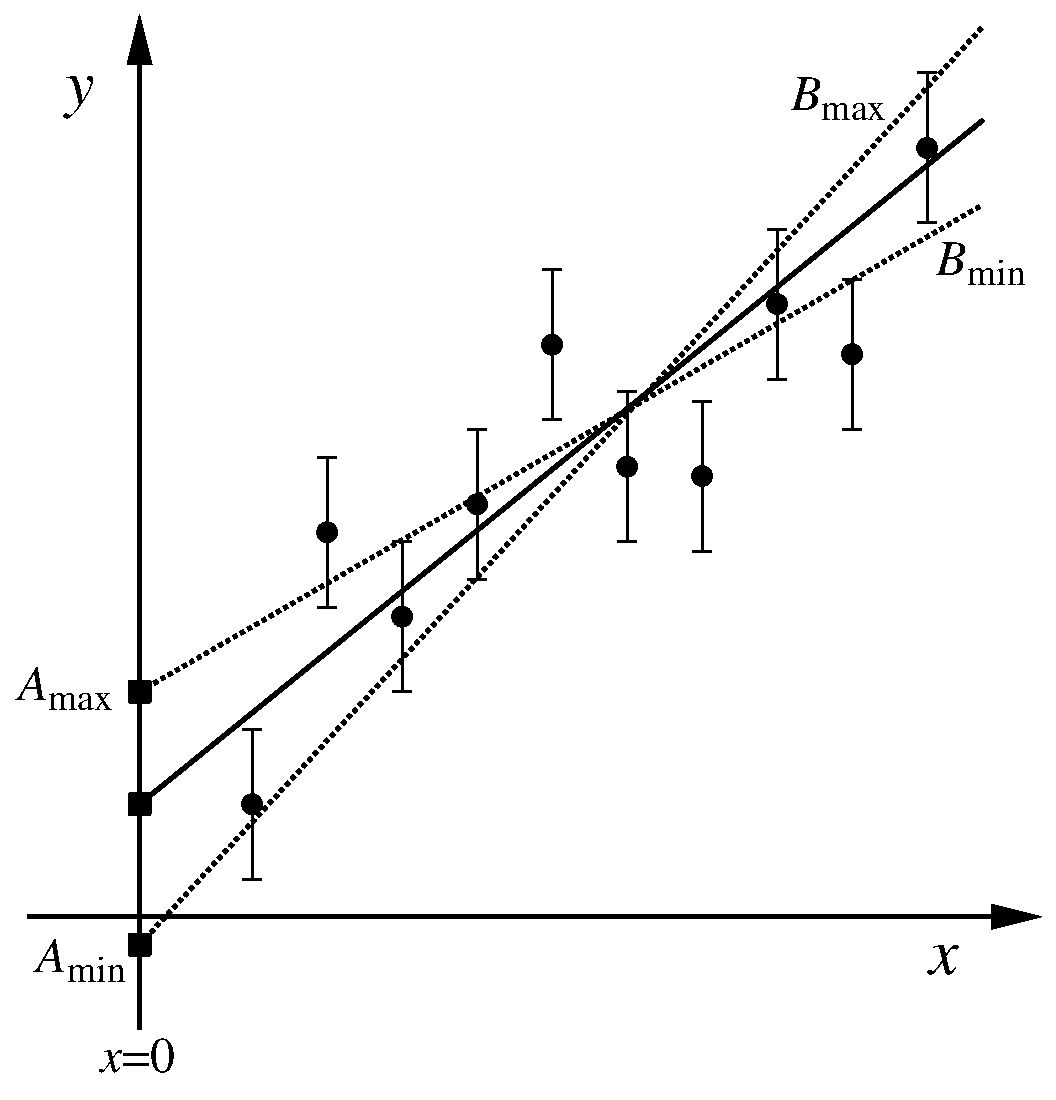
\includegraphics{gpherrB.eps}}}}
\end{center}
\caption{Finding the uncertainty in slope by hand (approximation)  \label{fig:slope}}
\end{figure}

 Our goal is to determine the parameters $A$ and $B$ from the
graph.  If the experimental data fall more or less on a straight
line (that is, it they satisfy the ``two-thirds criterion" for
a linear relationship), then we can obtain estimates for the
parameters $A$ and $B$ from the algebraic properties of a linear
function and the smooth curve (straight line) drawn through the
graphed data points.  For a linear relationship we note that any
two points $(x_{1}, y_{1})$ and $(x_{2}, y_{2})$ {\em on the line} can be used
to find an estimate for the slope of the line, $B$, since
\begin{eqnarray*}
y_{1} & = & A + Bx_{1} \\
y_{2} & = & A + Bx_{2}
\end{eqnarray*}
so that
\[
y_{2} - y_{1} = B(x_{2} - x_{1})
\]
 or
\[
B = {{y_{2} - y_{1}} \over {x_{2} - x_{1}}}
\]
Note that the units of $B$ are the units of $y/x$.

{\bf IMPORTANT: Do not} use two data points to find the slope!!
Rather use two well-separated points {\em on the line you have sketched}, which
represents information from {\em all} of the data points.

To estimate the $y$-intercept $A$, use one of the
following two methods: \begin{enumerate}
\item If the vertical line $x=0$ is physically on your graph,
then you can probably find where your sketched line intersects it.
The parameter $A$ is the
           value of $y$ where your sketched line
reaches $x=0$ (the ``$y$-intercept").
\item If the $y$-intercept is not on your graph (and very
           often it will not be), we simply note that the values
           for any point on the {\em line} can be used to solve for $A$,
           once we know the slope $B$, since $A = y_{i} - Bx_{i}$.
This method will usually be less accurate than the first.
\end{enumerate}

{\bf Example: }
     As an example let's try to see whether the temperature ($T$)
of a certain metal rod is linearly related to distance along the
rod ($d$).  The experimental observations are given in Table~\ref{table:temp}
and plotted in \ref{fig:temp}.
\begin{table}[h]
\begin{center}
\begin{tabular}{|ll|}
\hline
$d$ (cm) &\hspace{5pt} $T$ ($^{\circ}$C)  \\ \hline
 1 $\pm$ 0.01& \hspace{5pt} 16 $\pm$ 4  \\
2& \hspace{5pt} 18  \\
3& \hspace{5pt} 35  \\
4& \hspace{5pt} 44  \\
5& \hspace{5pt} 58  \\
6& \hspace{5pt} 62  \\
7& \hspace{5pt} 64  \\
8& \hspace{5pt} 70  \\  \hline
\end{tabular}
\end{center}
\caption{Sample data of temperature as a function of distance along a metal
         rod.  \label{table:temp}}
\end{table}


\begin{figure}[!hbt]     %Appendix C, Fig 2: temp vs distance
\begin{center}
{\resizebox{5in}{!}{\rotatebox{-90}{\includegraphics{temp_disB.ps}}}}
\end{center}
%\vspace{4in}
%\centerbmp{6.92in}{9in}{tempvsd.bmp}
%\special{ps:temp_dis.ps}
\caption{Graph of the data presented in Table~\protect\ref{table:temp}.
          \label{fig:temp}}
\end{figure}

It is straightforward to measure the slope $B$, as shown above.  The
uncertainty in the slope can be
estimated from the ``best" line (as judged by eye), and from
upper and lower outer limits of possible slopes that might
work, (for example, the dotted lines in Fig.~\ref{fig:slope} above).
As an exercise, try to find $A$, $B$ and their
uncertainties; you should find something like
\begin{equation}
A  =  8 \pm 4 \;^{\circ}\mbox{C}, \ \ \ \
B   =  8 \pm 1 \;^{\circ}\mbox{C/cm}
\end{equation}

\section*{Graphical Analysis: Curves}


    It is fairly easy to determine whether a set of data lies on
a straight line.  But what if it doesn't --- what if the smooth line
drawn through a set of data in fact curves?  How can we
decide whether that curve represents a quadratic, or a cubic, or
some other function?  The next two sections will show
how two fairly common functional forms, power laws and
exponentials, can be transformed so that they look like straight
lines, and hence can be easily identified and analyzed.  The
same sort of transformation process applies to many functional forms.

    These two sections will be primarily concerned with graphical
analysis, but we can also use the method of least squares to find the
``best" values for the function parameters and their
uncertainties---see Appendix D.

\paragraph*{2.  Exponential Function}
\label{exprel}
An exponential function takes the form
\begin{equation}
y = A\, e^{Bx}     \label{eq:c4}
\end{equation}
where $e$ is the base of natural logarithms.

This function is not linear, and hence will
show some curvature on a linear graph.
%\subsection*{Exponential Graphical Analysis}
     To  analyze exponential relationships graphically, we
begin by taking the logarithm of both sides of  the above
exponential equation, Eq.~\ref{eq:c4}.
%\begin{equation}
%y = A\, e^{Bx}  \label{eq:c4a}
%\end{equation}
Recall that for natural logarithms,
\[
\ln e^{t}  = t
\]
and
\[
\ln AB = \ln A + \ln B .
\]
So taking the the natural logarithm of both sides of
Eq.~\ref{eq:c4}, we obtain
\begin{equation}
\ln y = \ln(A \, e^{Bx}) = \ln A + \ln \, e^{Bx}
   = \ln A + Bx   \label{eq:c5}
\end{equation}
If we now define $Y \equiv \ln y$ and $C \equiv \ln A$, this
equation becomes 
\begin{equation}
Y = C + Bx \label{eq:transform_line}
\end{equation}

which is the equation of a straight line with slope $B$ and
intercept $C$!  Thus if we plot $Y$ versus $x$ (that is,
$\ln y$ versus $x$) and obtain a straight line, we may infer that our
data can be described by an exponential function.  A graph of
$\ln y$ versus $x$ is often called a semi-log graph.

Note that we have used natural (base $e$) logarithms in this section
instead common (base 10) logarithms.  Either will linearize an exponential
relationship
(although natural logarithms are widely used in science and engineering).
  In either case,
it is easy to find the logarithms, either with a calculator or a
spreadsheet (such as Excel\footnote{
In Excel {\tt log10()}=$\log_{10}()$ and {\tt ln()}=$\log_e()$.
 {\tt log()} by itself is ambiguous: in Excel it is $\log_{10}()$
but in most computer languages it is $\log_e()$.}).

Suppose, then, that our data can be described by a straight line
on a semi-log graph.  We can find the slope $B$ and intercept $C$
from this second graph, exactly as described above.
Thus, the slope can be calculated by picking two points
on the line of the graph of $\ln y$ vs.\ $x$ and calculating
\begin{equation}
B = {{Y_{2} - Y_{1}} \over {x_{2} - x_{1}}} = {{\ln y_{2} - \ln y_{1}}
           \over {x_{2} - x_{1}}} = 
{\ln\left(y_{2}/y_{1}\right) \over x_{2} - x_{1}}  \label{eq:cnew}
\end{equation}
Note that the units of $B$ are the units of $1/x$, since the results of the 
standard functions---including $\ln()$---never have units. 

The intercept $C$ can likewise be easily found, and once we have it,
we can find the parameter $A$ by observing that

%\begin{enumerate}
%\item A graph of the calculated values of $\ln y$ vs.\ $x$ on
%           linear graph paper (see Fig.~\ref{fig:c3b} and Fig.~\ref{fig:c3b1}).
%\item A graph of $y$ vs.\ $x$ on semi-log paper which has the
%           $y$-axis stretched in such a way as to do the linear
%           transformation for us (see Fig.~\ref{fig:c3c}).
%\end{enumerate}
%
\begin{equation}
C = \ln A  \qquad \mbox{or} \qquad  A = e^{C} \label{eq:transformC}
\end{equation}
The above equations disguise the units of $A$, however if you return to Eq.~\ref{eq:c4}
and recall that ``the 
standard functions---including $\exp(Bx)=e^{Bx}$---never have units"
it should be clear that $A$ has the same units as $y$.

Thus we have found the parameters $A$ and $B$ that describe our
exponential function.

%In addition an
%exponential has a constant doubling interval and this property
%can be used to distinguish it from a power relationship.  To
%calculate the doubling interval of a curve, pick some small $y$
%value (say $y_{1}$) and note the $x$ coordinate (say $x_{1}$).  Then find the
%$x$ coordinates where $y = 2y_{1}$ and $4y_{1}$ (call them $x_{2}$ and $x_{4}$).
%If
%\[
%x_{2} - x_{1} \approx x_{4} - x_{2}
%\]
%then the doubling interval is approximately constant.  For
%example, find the doubling interval for the data for altitude, $H$,
%versus  given in the Table~\ref{table:c3a} and
%plotted in Fig.~\ref{fig:c3a} and Fig.~\ref{fig:c3a1}.

{\bf Example: }
As an example, consider the data for atmospheric pressure, $P$,
versus altitude, $H$, given in the following table.
% atmospheric pressure, $P$, given in the Table~\ref{table:c3a} and
%plotted in Fig.~\ref{fig:c3a} and Fig.~\ref{fig:c3a1
For this data set the uncertainty in pressure, $\delta P$, is 0.03~bar
and the uncertainty in height is `negligible' (i.e., assumed small enough
not to matter).

\begin{table}[h]
\begin{center}
\begin{tabular}{|rlrcc|}
\hline
$H$ (km) & $P$ (bars) & $\ln P$ & $\ln (P + \delta P)$ & $\ln (P - \delta P)$ \\
 \hline
0.0 \hspace{6pt}  & 1.00 $\pm$ 0.03 & 0.00    & +0.03     &  $-$0.03\\
2.0 \hspace{6pt}  & 0.75            & $-$0.29 & $-$0.25   &  $-$0.33 \\
4.0 \hspace{6pt}  &     0.60        & $-$0.51 &   $-$0.46 &  $-$0.56 \\
5.0 \hspace{6pt}  &     0.48        & $-$0.73 &   $-$0.67 &  $-$0.80 \\
7.5 \hspace{6pt}  &   0.37          & $-$0.99 &   $-$0.92 &  $-$1.08  \\
10.0 \hspace{6pt} &   0.27          & $-$1.31 &   $-$1.20 &  $-$1.43 \\
15.0 \hspace{6pt} &     0.14        & $-$1.97 &   $-$1.77 &  $-$2.21 \\
20.0 \hspace{6pt} &     0.07        & $-$2.66 &   $-$2.30 &  $-$3.22 \\
\hline
\end{tabular}
\end{center}
\caption{Sample data of pressure vs.\ height in the atmosphere.
     \label{table:pressure}}
\end{table}

Please inspect carefully the table, and the two graphs on the following
page.  The first graph (a straightforward plot of $P$ vs.\ $H$)
shows a curve.  The second is a semi-log graph (that
is, a graph of $\ln(P)$ vs.\ $H$) that shows a straight line.  
(Note that the log scale
changes the appearance of the error bars: they are not symmetrical
and the bar size has changed from the ``normal" plot. That final error bar
ranges from $\ln(0.04)=-3.22$ to $\ln(0.10)=-2.30$ with anchor at $\ln(0.07)=-2.66$.)  
Since this second
graph is linear, we may infer that these data are consistent with an
exponential function.  As an exercise, see if you can determine the
parameters $A$ and $B$ in Eq.~\ref{eq:c4}, above by making your own
semi-log graph and finding the slope and intercept.

\newpage

\begin{figure}[!hbt]    %linear graph of pressure vs altitude
\begin{center}
{\resizebox{5in}{!}{\rotatebox{-90}{\includegraphics{pressureB.ps}}}}
\end{center}
%\vspace{4in}
%\centerbmp{6.94in}{9in}{pressure.bmp}
%\special{ps:pressure.ps}
\caption{Graph of the data presented in Table~\protect\ref{table:pressure}.
          \label{fig:pressure}}
\end{figure}

\begin{figure}[!hbt]   %semi-log graph of pressure vs altitude
\begin{center}
{\resizebox{5in}{!}{\rotatebox{-90}{\includegraphics{pressure_logB.ps}}}}
\end{center}
%\vspace{4in}
%\special{ps:pressure_log.ps}
\caption{Semi-log graph of the data presented in Table~\protect\ref{table:pressure}.
          \label{fig:pressure_log}}
\end{figure}



\paragraph*{3. Power Law}


    By a power law we mean an equation of the form
\begin{equation}
y = Ax^{B}  \label{eq:c3}
\end{equation}
If $B = 2$, for example, we have a quadratic.
In general, a power law equation shows curvature.

     Once again we begin by taking the natural logarithm of both sides of the
power-law equation. 
%\[
%y = Ax^{B}.
%\]
As we shall see, this step will ``linearize'' the equation --- 
the technique is similar to the one we used for
exponentials.  Taking the logarithm of both sides of the equation, we
obtain
\[
\ln y = \ln (Ax^{B}).
\]
And since
\begin{eqnarray*}
\ln (Ax^{B}) & = & \ln A + \ln (x^{B}) \\
              & = & \ln A + B \: \ln x
\end{eqnarray*}
we obtain the result
\[
\ln y = \ln A + B \: \ln x .
\]
If we define two new variables $Y \equiv \ln y$ and $X \equiv \ln
x$ and
a new constant $C \equiv \ln A$ then we obtain the transformed
equation
\[
Y = C + BX
\]
which is the equation of a straight line!

  Therefore, to find out if our data are consistent with a power law,
we make a graph of
$Y$ versus $X$ (that is, $\ln y$ versus $\ln x$).  Such a graph
is often called a ``log-log'' graph.  If our data lie along a straight
line on the log-log plot, then we can say that those data are consistent
with a power law.

We can find the slope $B$ and
the intercept $C= \ln A$ as before.  In this case, the slope $B$ is
given by
\[
B = {{Y_{2} - Y_{1}} \over {X_{2} - X_{1}}} =
    {{\ln y_{2} - \ln y_{1}} \over {\ln x_{2} - \ln x_{1}}} =
{\ln\left(y_2/y_1\right) \over \ln\left(x_2/x_1\right) }
\]
Note that this $B$ has no units.

We can find the parameter $A$ by noting that the intercept $C$ is
given by $C = \ln A$ (or $A = {e}^{C}$).  
Note that the units of $A$ are the units of $y/x^B$.
Thus, we have
recovered the parameters $A$ and $B$ for the power law function.

%There are two ways to make this graph:
%\begin{enumerate}
%\item We could calculate $\log y_{i}$ and $\log x_{i}$ for each data
%           point and plot them on linear paper (see Fig.~\ref{fig:c2b},
%Fig.~\ref{fig:c2b1} and Table~\ref{table:c2b}); if we use this procedure, we must
%           plot the error bars by plotting $\log (y + \delta y)$ and
%           $\log (y - \delta y)$ for each point, since of course
%           $\log(y + \delta y) \neq \log y + \log \delta y$.
%\item Use special graph paper called log-log paper where the
%           scales have been stretched to do the linear
%           transformation for us and plot the data points
%           directly (see Fig.~\ref{fig:c2c}).  (We do not especially
%           recommend this option --- the first method is generally
%           more convenient.)  In either case the $y$-intercept ($C$)
%           and the slope ($B$) can be found from the procedures
%           outlined above.
%\end{enumerate}

{\bf Example: } 
As an example, consider
 the data presented in
Table~\ref{table:speed} of the speed of sound in a gas, $V$, versus
the
molecular weight $M$.  These data are plotted in Figs.~\ref{fig:speed},
\ref{fig:speed_log}, and \ref{fig:speed_true_log}.


\begin{table}[hbt!]
\begin{center}
\begin{tabular}{|rcrcccccc|}
\hline
$M$ & \hspace{6pt} & $V$(m/s) & \hspace{6pt}
& $\ln M$ & \hspace{6pt} & $\ln V$ & $\ln(V + \delta V)$ & $\ln (V
- \delta V)$ \\ \hline

2  & & 1270 $\pm$ 20 &  & 0.69 & &  7.15 & 7.16 & 7.13  \\
4  & & 890  $\pm$ 20 &  & 1.39 & &  6.79 & 6.81 & 6.77  \\
14 & & 477  $\pm$ 20 &  & 2.64 & &  6.17 & 6.21 & 6.12  \\
16 & & 432  $\pm$ 20 &  & 2.77 & &  6.07 & 6.11 & 6.02  \\
29 & & 344  $\pm$ 20 &  & 3.37 & &  5.84 & 5.90 & 5.78  \\
32 & & 317  $\pm$ 20 &  & 3.47 & &  5.76 & 5.82 & 5.69  \\
44 & & 238  $\pm$ 20 &  & 3.78 & &  5.47 & 5.55 & 5.38  \\ \hline
\end{tabular}
\end{center}
\caption{Sample data of the speed of sound in a gas vs.\ molecular weight of
the gas.  \label{table:speed}}
\end{table}

The first graph is shows that the speed of sound is a rapidly
decreasing function of the molecular weight of a gas. The second one
is a log-log graph of the same data,
on which the data fall roughly on a straight line.  In this case,
therefore, we infer that the data are consistent with a power law (in
this case, a power law with a negative exponent, since the speed
decreases as the molecular weight increases and hence the slope
is negative.)

As an exercise, see if you can find the parameters $A$ and $B$ in
Eq.~\ref{eq:c3} for
these data, by making your own log-log graph and finding the slope and
intercept.

\begin{figure}[!hbt]    %linear graph of speed vs molecular weight
\begin{center}
{\resizebox{5in}{!}{\rotatebox{-90}{\includegraphics{speedB.ps}}}}
\end{center}
%\vspace{4in}
%\special{ps:speed.ps}
\caption{Graph of the data presented in Table~\protect\ref{table:speed}.
          \label{fig:speed}}
\end{figure}

\begin{figure}[!hbt]   %semi-log graph of pressure vs altitude
\begin{center}
{\resizebox{5in}{!}{\rotatebox{-90}{\includegraphics{speed_log_logB.ps}}}}
\end{center}
%\vspace{4in}
%\special{ps:speed_log.ps}
\caption{Log-log graph of the data presented in Table~\protect\ref{table:speed}.
          \label{fig:speed_log}}
\end{figure}

\begin{figure}[!hbt]   %semi-log graph of pressure vs altitude
\begin{center}
{\resizebox{5in}{!}{\rotatebox{-90}{\includegraphics{speed_true_log_logB.ps}}}}
\end{center}
%\vspace{4in}
%\special{ps:speed_log.ps}
\caption{With a ``log  scale" the labels are the actual values
but the tic marks are spaced according to the logarithm. 
These scales make locating points easy and is the preferred
way of making a log-log plot.
          \label{fig:speed_true_log}}
\end{figure}

%\vspace{4in}






